\documentclass[1p]{elsarticle_modified}
%\bibliographystyle{elsarticle-num}

%\usepackage[colorlinks]{hyperref}
%\usepackage{abbrmath_seonhwa} %\Abb, \Ascr, \Acal ,\Abf, \Afrak
\usepackage{amsfonts}
\usepackage{amssymb}
\usepackage{amsmath}
\usepackage{amsthm}
\usepackage{scalefnt}
\usepackage{amsbsy}
\usepackage{kotex}
\usepackage{caption}
\usepackage{subfig}
\usepackage{color}
\usepackage{graphicx}
\usepackage{xcolor} %% white, black, red, green, blue, cyan, magenta, yellow
\usepackage{float}
\usepackage{setspace}
\usepackage{hyperref}

\usepackage{tikz}
\usetikzlibrary{arrows}

\usepackage{multirow}
\usepackage{array} % fixed length table
\usepackage{hhline}

%%%%%%%%%%%%%%%%%%%%%
\makeatletter
\renewcommand*\env@matrix[1][\arraystretch]{%
	\edef\arraystretch{#1}%
	\hskip -\arraycolsep
	\let\@ifnextchar\new@ifnextchar
	\array{*\c@MaxMatrixCols c}}
\makeatother %https://tex.stackexchange.com/questions/14071/how-can-i-increase-the-line-spacing-in-a-matrix
%%%%%%%%%%%%%%%

\usepackage[normalem]{ulem}

\newcommand{\msout}[1]{\ifmmode\text{\sout{\ensuremath{#1}}}\else\sout{#1}\fi}
%SOURCE: \msout is \stkout macro in https://tex.stackexchange.com/questions/20609/strikeout-in-math-mode

\newcommand{\cancel}[1]{
	\ifmmode
	{\color{red}\msout{#1}}
	\else
	{\color{red}\sout{#1}}
	\fi
}

\newcommand{\add}[1]{
	{\color{blue}\uwave{#1}}
}

\newcommand{\replace}[2]{
	\ifmmode
	{\color{red}\msout{#1}}{\color{blue}\uwave{#2}}
	\else
	{\color{red}\sout{#1}}{\color{blue}\uwave{#2}}
	\fi
}

\newcommand{\Sol}{\mathcal{S}} %segment
\newcommand{\D}{D} %diagram
\newcommand{\A}{\mathcal{A}} %arc


%%%%%%%%%%%%%%%%%%%%%%%%%%%%%5 test

\def\sl{\operatorname{\textup{SL}}(2,\Cbb)}
\def\psl{\operatorname{\textup{PSL}}(2,\Cbb)}
\def\quan{\mkern 1mu \triangleright \mkern 1mu}

\theoremstyle{definition}
\newtheorem{thm}{Theorem}[section]
\newtheorem{prop}[thm]{Proposition}
\newtheorem{lem}[thm]{Lemma}
\newtheorem{ques}[thm]{Question}
\newtheorem{cor}[thm]{Corollary}
\newtheorem{defn}[thm]{Definition}
\newtheorem{exam}[thm]{Example}
\newtheorem{rmk}[thm]{Remark}
\newtheorem{alg}[thm]{Algorithm}

\newcommand{\I}{\sqrt{-1}}
\begin{document}

%\begin{frontmatter}
%
%\title{Boundary parabolic representations of knots up to 8 crossings}
%
%%% Group authors per affiliation:
%\author{Yunhi Cho} 
%\address{Department of Mathematics, University of Seoul, Seoul, Korea}
%\ead{yhcho@uos.ac.kr}
%
%
%\author{Seonhwa Kim} %\fnref{s_kim}}
%\address{Center for Geometry and Physics, Institute for Basic Science, Pohang, 37673, Korea}
%\ead{ryeona17@ibs.re.kr}
%
%\author{Hyuk Kim}
%\address{Department of Mathematical Sciences, Seoul National University, Seoul 08826, Korea}
%\ead{hyukkim@snu.ac.kr}
%
%\author{Seokbeom Yoon}
%\address{Department of Mathematical Sciences, Seoul National University, Seoul, 08826,  Korea}
%\ead{sbyoon15@snu.ac.kr}
%
%\begin{abstract}
%We find all boundary parabolic representation of knots up to 8 crossings.
%
%\end{abstract}
%\begin{keyword}
%    \MSC[2010] 57M25 
%\end{keyword}
%
%\end{frontmatter}

%\linenumbers
%\tableofcontents
%
\newcommand\colored[1]{\textcolor{white}{\rule[-0.35ex]{0.8em}{1.4ex}}\kern-0.8em\color{red} #1}%
%\newcommand\colored[1]{\textcolor{white}{ #1}\kern-2.17ex	\textcolor{white}{ #1}\kern-1.81ex	\textcolor{white}{ #1}\kern-2.15ex\color{red}#1	}

{\Large $\underline{12a_{0953}~(K12a_{0953})}$}

\setlength{\tabcolsep}{10pt}
\renewcommand{\arraystretch}{1.6}
\vspace{1cm}\begin{tabular}{m{100pt}>{\centering\arraybackslash}m{274pt}}
\multirow{5}{120pt}{
	\centering
	\includegraphics[width=112pt]{../../../GIT/diagram.site/Diagrams/png/1754_12a_0953.png}\\
\ \ \ A knot diagram\footnotemark}&
\allowdisplaybreaks
\textbf{Linearized knot diagam} \\
\cline{2-2}
 &
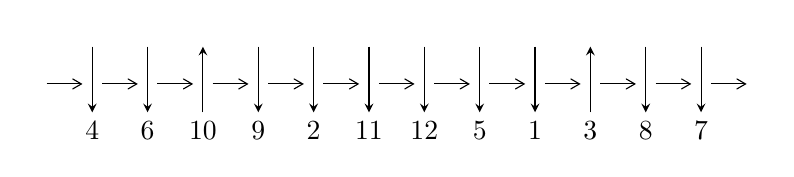
\begin{tikzpicture}[x=20pt, y=17pt]
	% nodes
	\node (C0) at (0, 0) {};
	\node (C1) at (1, 0) {};
	\node (C1U) at (1, +1) {};
	\node (C1D) at (1, -1) {4};

	\node (C2) at (2, 0) {};
	\node (C2U) at (2, +1) {};
	\node (C2D) at (2, -1) {6};

	\node (C3) at (3, 0) {};
	\node (C3U) at (3, +1) {};
	\node (C3D) at (3, -1) {10};

	\node (C4) at (4, 0) {};
	\node (C4U) at (4, +1) {};
	\node (C4D) at (4, -1) {9};

	\node (C5) at (5, 0) {};
	\node (C5U) at (5, +1) {};
	\node (C5D) at (5, -1) {2};

	\node (C6) at (6, 0) {};
	\node (C6U) at (6, +1) {};
	\node (C6D) at (6, -1) {11};

	\node (C7) at (7, 0) {};
	\node (C7U) at (7, +1) {};
	\node (C7D) at (7, -1) {12};

	\node (C8) at (8, 0) {};
	\node (C8U) at (8, +1) {};
	\node (C8D) at (8, -1) {5};

	\node (C9) at (9, 0) {};
	\node (C9U) at (9, +1) {};
	\node (C9D) at (9, -1) {1};

	\node (C10) at (10, 0) {};
	\node (C10U) at (10, +1) {};
	\node (C10D) at (10, -1) {3};

	\node (C11) at (11, 0) {};
	\node (C11U) at (11, +1) {};
	\node (C11D) at (11, -1) {8};

	\node (C12) at (12, 0) {};
	\node (C12U) at (12, +1) {};
	\node (C12D) at (12, -1) {7};
	\node (C13) at (13, 0) {};

	% arrows
	\draw[->,>={angle 60}]
	(C0) edge (C1) (C1) edge (C2) (C2) edge (C3) (C3) edge (C4) (C4) edge (C5) (C5) edge (C6) (C6) edge (C7) (C7) edge (C8) (C8) edge (C9) (C9) edge (C10) (C10) edge (C11) (C11) edge (C12) (C12) edge (C13) ;	\draw[->,>=stealth]
	(C1U) edge (C1D) (C2U) edge (C2D) (C3D) edge (C3U) (C4U) edge (C4D) (C5U) edge (C5D) (C6U) edge (C6D) (C7U) edge (C7D) (C8U) edge (C8D) (C9U) edge (C9D) (C10D) edge (C10U) (C11U) edge (C11D) (C12U) edge (C12D) ;
	\end{tikzpicture} \\
\hhline{~~} \\& 
\textbf{Solving Sequence} \\ \cline{2-2} 
 &
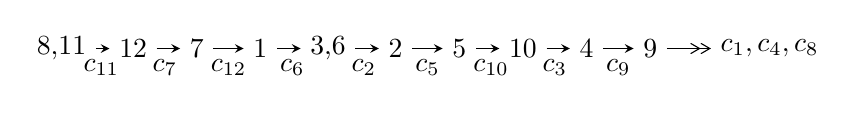
\begin{tikzpicture}[x=23pt, y=7pt]
	% node
	\node (A0) at (-1/8, 0) {8,11};
	\node (A1) at (1, 0) {12};
	\node (A2) at (2, 0) {7};
	\node (A3) at (3, 0) {1};
	\node (A4) at (65/16, 0) {3,6};
	\node (A5) at (41/8, 0) {2};
	\node (A6) at (49/8, 0) {5};
	\node (A7) at (57/8, 0) {10};
	\node (A8) at (65/8, 0) {4};
	\node (A9) at (73/8, 0) {9};
	\node (C1) at (1/2, -1) {$c_{11}$};
	\node (C2) at (3/2, -1) {$c_{7}$};
	\node (C3) at (5/2, -1) {$c_{12}$};
	\node (C4) at (7/2, -1) {$c_{6}$};
	\node (C5) at (37/8, -1) {$c_{2}$};
	\node (C6) at (45/8, -1) {$c_{5}$};
	\node (C7) at (53/8, -1) {$c_{10}$};
	\node (C8) at (61/8, -1) {$c_{3}$};
	\node (C9) at (69/8, -1) {$c_{9}$};
	\node (A10) at (11, 0) {$c_{1},c_{4},c_{8}$};

	% edge
	\draw[->,>=stealth]	
	(A0) edge (A1) (A1) edge (A2) (A2) edge (A3) (A3) edge (A4) (A4) edge (A5) (A5) edge (A6) (A6) edge (A7) (A7) edge (A8) (A8) edge (A9) ;
	\draw[->>,>={angle 60}]	
	(A9) edge (A10);
\end{tikzpicture} \\ 

\end{tabular} \\

\footnotetext{
The image of knot diagram is generated by the software ``\textbf{Draw programme}" developed by Andrew Bartholomew(\url{http://www.layer8.co.uk/maths/draw/index.htm\#Running-draw}), where we modified some parts for our purpose(\url{https://github.com/CATsTAILs/LinksPainter}).
}\phantom \\ \newline 
\centering \textbf{Ideals for irreducible components\footnotemark of $X_{\text{par}}$} 
 
\begin{align*}
I^u_{1}&=\langle 
-6.38203\times10^{172} u^{109}-1.26988\times10^{173} u^{108}+\cdots+7.34383\times10^{172} b-6.55266\times10^{173},\\
\phantom{I^u_{1}}&\phantom{= \langle  }-8.43112\times10^{173} u^{109}-1.62348\times10^{174} u^{108}+\cdots+8.07821\times10^{173} a-2.66760\times10^{175},\\
\phantom{I^u_{1}}&\phantom{= \langle  }u^{110}+u^{109}+\cdots+278 u+11\rangle \\
I^u_{2}&=\langle 
u^{17}-3 u^{16}+\cdots-4 u^2+b,\;-2 u^{17}+3 u^{16}+\cdots+a+3,\;u^{18}-2 u^{17}+\cdots-2 u+1\rangle \\
\\
\end{align*}
\raggedright * 2 irreducible components of $\dim_{\mathbb{C}}=0$, with total 128 representations.\\
\footnotetext{All coefficients of polynomials are rational numbers. But the coefficients are sometimes approximated in decimal forms when there is not enough margin.}
\newpage
\renewcommand{\arraystretch}{1}
\centering \section*{I. $I^u_{1}= \langle -6.38\times10^{172} u^{109}-1.27\times10^{173} u^{108}+\cdots+7.34\times10^{172} b-6.55\times10^{173},\;-8.43\times10^{173} u^{109}-1.62\times10^{174} u^{108}+\cdots+8.08\times10^{173} a-2.67\times10^{175},\;u^{110}+u^{109}+\cdots+278 u+11 \rangle$}
\flushleft \textbf{(i) Arc colorings}\\
\begin{tabular}{m{7pt} m{180pt} m{7pt} m{180pt} }
\flushright $a_{8}=$&$\begin{pmatrix}0\\u\end{pmatrix}$ \\
\flushright $a_{11}=$&$\begin{pmatrix}1\\0\end{pmatrix}$ \\
\flushright $a_{12}=$&$\begin{pmatrix}1\\u^2\end{pmatrix}$ \\
\flushright $a_{7}=$&$\begin{pmatrix}u\\u^3+u\end{pmatrix}$ \\
\flushright $a_{1}=$&$\begin{pmatrix}u^2+1\\u^4+2 u^2\end{pmatrix}$ \\
\flushright $a_{3}=$&$\begin{pmatrix}1.04369 u^{109}+2.00971 u^{108}+\cdots+410.322 u+33.0222\\0.869033 u^{109}+1.72918 u^{108}+\cdots+215.319 u+8.92267\end{pmatrix}$ \\
\flushright $a_{6}=$&$\begin{pmatrix}u^3+2 u\\u^3+u\end{pmatrix}$ \\
\flushright $a_{2}=$&$\begin{pmatrix}0.493453 u^{109}-0.225088 u^{108}+\cdots+53.1992 u+18.7418\\2.24757 u^{109}+2.09482 u^{108}+\cdots+140.726 u+5.47659\end{pmatrix}$ \\
\flushright $a_{5}=$&$\begin{pmatrix}-0.161257 u^{109}-0.431389 u^{108}+\cdots-177.617 u-21.5655\\2.15866 u^{109}+1.69325 u^{108}+\cdots+122.861 u+3.85095\end{pmatrix}$ \\
\flushright $a_{10}=$&$\begin{pmatrix}-0.852999 u^{109}-1.28126 u^{108}+\cdots+26.0895 u+12.5914\\0.614891 u^{109}-2.63198 u^{108}+\cdots-444.568 u-17.4155\end{pmatrix}$ \\
\flushright $a_{4}=$&$\begin{pmatrix}1.34925 u^{109}-1.78726 u^{108}+\cdots-249.644 u+13.2485\\2.96760 u^{109}+2.44514 u^{108}+\cdots+112.628 u+4.40678\end{pmatrix}$ \\
\flushright $a_{9}=$&$\begin{pmatrix}-1.42892 u^{109}-1.87328 u^{108}+\cdots-8.25883 u+11.7779\\0.444642 u^{109}-4.02819 u^{108}+\cdots-668.229 u-26.2983\end{pmatrix}$\\&\end{tabular}
\flushleft \textbf{(ii) Obstruction class $= -1$}\\~\\
\flushleft \textbf{(iii) Cusp Shapes $= -3.06007 u^{109}-8.46109 u^{108}+\cdots-680.493 u-29.6266$}\\~\\
\newpage\renewcommand{\arraystretch}{1}
\flushleft \textbf{(iv) u-Polynomials at the component}\newline \\
\begin{tabular}{m{50pt}|m{274pt}}
Crossings & \hspace{64pt}u-Polynomials at each crossing \\
\hline $$\begin{aligned}c_{1}\end{aligned}$$&$\begin{aligned}
&u^{110}-12 u^{109}+\cdots+30 u-1
\end{aligned}$\\
\hline $$\begin{aligned}c_{2},c_{5}\end{aligned}$$&$\begin{aligned}
&u^{110}+u^{109}+\cdots+44559 u+1087
\end{aligned}$\\
\hline $$\begin{aligned}c_{3},c_{10}\end{aligned}$$&$\begin{aligned}
&u^{110}+u^{109}+\cdots-21765 u+12969
\end{aligned}$\\
\hline $$\begin{aligned}c_{4},c_{8}\end{aligned}$$&$\begin{aligned}
&u^{110}+4 u^{109}+\cdots+1542 u+279
\end{aligned}$\\
\hline $$\begin{aligned}c_{6}\end{aligned}$$&$\begin{aligned}
&u^{110}- u^{109}+\cdots+10791316 u+468259
\end{aligned}$\\
\hline $$\begin{aligned}c_{7},c_{11},c_{12}\end{aligned}$$&$\begin{aligned}
&u^{110}+u^{109}+\cdots+278 u+11
\end{aligned}$\\
\hline $$\begin{aligned}c_{9}\end{aligned}$$&$\begin{aligned}
&u^{110}+6 u^{109}+\cdots+37 u^2-1
\end{aligned}$\\
\hline
\end{tabular}\\~\\
\newpage\renewcommand{\arraystretch}{1}
\flushleft \textbf{(v) Riley Polynomials at the component}\newline \\
\begin{tabular}{m{50pt}|m{274pt}}
Crossings & \hspace{64pt}Riley Polynomials at each crossing \\
\hline $$\begin{aligned}c_{1}\end{aligned}$$&$\begin{aligned}
&y^{110}-10 y^{109}+\cdots-82 y+1
\end{aligned}$\\
\hline $$\begin{aligned}c_{2},c_{5}\end{aligned}$$&$\begin{aligned}
&y^{110}-85 y^{109}+\cdots-674723791 y+1181569
\end{aligned}$\\
\hline $$\begin{aligned}c_{3},c_{10}\end{aligned}$$&$\begin{aligned}
&y^{110}+79 y^{109}+\cdots-4284448371 y+168194961
\end{aligned}$\\
\hline $$\begin{aligned}c_{4},c_{8}\end{aligned}$$&$\begin{aligned}
&y^{110}+56 y^{109}+\cdots+3663144 y+77841
\end{aligned}$\\
\hline $$\begin{aligned}c_{6}\end{aligned}$$&$\begin{aligned}
&y^{110}-53 y^{109}+\cdots-63491367640358 y+219266491081
\end{aligned}$\\
\hline $$\begin{aligned}c_{7},c_{11},c_{12}\end{aligned}$$&$\begin{aligned}
&y^{110}+95 y^{109}+\cdots-35726 y+121
\end{aligned}$\\
\hline $$\begin{aligned}c_{9}\end{aligned}$$&$\begin{aligned}
&y^{110}+102 y^{108}+\cdots-74 y+1
\end{aligned}$\\
\hline
\end{tabular}\\~\\
\newpage\flushleft \textbf{(vi) Complex Volumes and Cusp Shapes}
$$\begin{array}{c|c|c}  
\text{Solutions to }I^u_{1}& \I (\text{vol} + \sqrt{-1}CS) & \text{Cusp shape}\\
 \hline 
\begin{aligned}
u &= \phantom{-}1.050010 + 0.171279 I \\
a &= -0.33161 - 1.70441 I \\
b &= \phantom{-}0.166210 - 1.222580 I\end{aligned}
 & -6.04457 - 0.70873 I & \phantom{-0.000000 } 0 \\ \hline\begin{aligned}
u &= \phantom{-}1.050010 - 0.171279 I \\
a &= -0.33161 + 1.70441 I \\
b &= \phantom{-}0.166210 + 1.222580 I\end{aligned}
 & -6.04457 + 0.70873 I & \phantom{-0.000000 } 0 \\ \hline\begin{aligned}
u &= -0.891130 + 0.230513 I \\
a &= \phantom{-}0.41804 - 2.22971 I \\
b &= -0.46710 - 1.48139 I\end{aligned}
 & -6.4223 + 13.5900 I & \phantom{-0.000000 } 0 \\ \hline\begin{aligned}
u &= -0.891130 - 0.230513 I \\
a &= \phantom{-}0.41804 + 2.22971 I \\
b &= -0.46710 + 1.48139 I\end{aligned}
 & -6.4223 - 13.5900 I & \phantom{-0.000000 } 0 \\ \hline\begin{aligned}
u &= -0.996011 + 0.461027 I \\
a &= -0.52667 + 1.36913 I \\
b &= \phantom{-}0.120769 + 1.233970 I\end{aligned}
 & -6.47998 + 3.06048 I & \phantom{-0.000000 } 0 \\ \hline\begin{aligned}
u &= -0.996011 - 0.461027 I \\
a &= -0.52667 - 1.36913 I \\
b &= \phantom{-}0.120769 - 1.233970 I\end{aligned}
 & -6.47998 - 3.06048 I & \phantom{-0.000000 } 0 \\ \hline\begin{aligned}
u &= \phantom{-}0.420393 + 1.023990 I \\
a &= \phantom{-}0.714613 + 0.842054 I \\
b &= \phantom{-}0.34795 + 1.51364 I\end{aligned}
 & -7.29839 + 2.86587 I & \phantom{-0.000000 } 0 \\ \hline\begin{aligned}
u &= \phantom{-}0.420393 - 1.023990 I \\
a &= \phantom{-}0.714613 - 0.842054 I \\
b &= \phantom{-}0.34795 - 1.51364 I\end{aligned}
 & -7.29839 - 2.86587 I & \phantom{-0.000000 } 0 \\ \hline\begin{aligned}
u &= \phantom{-}0.196637 + 1.125380 I \\
a &= -0.332867 - 0.830505 I \\
b &= \phantom{-}0.941856 + 0.626895 I\end{aligned}
 & \phantom{-}1.93918 + 4.29723 I & \phantom{-0.000000 } 0 \\ \hline\begin{aligned}
u &= \phantom{-}0.196637 - 1.125380 I \\
a &= -0.332867 + 0.830505 I \\
b &= \phantom{-}0.941856 - 0.626895 I\end{aligned}
 & \phantom{-}1.93918 - 4.29723 I & \phantom{-0.000000 } 0\\
 \hline 
 \end{array}$$\newpage$$\begin{array}{c|c|c}  
\text{Solutions to }I^u_{1}& \I (\text{vol} + \sqrt{-1}CS) & \text{Cusp shape}\\
 \hline 
\begin{aligned}
u &= -0.560509 + 1.002830 I \\
a &= \phantom{-}0.654267 - 0.947169 I \\
b &= \phantom{-}0.36228 - 1.43029 I\end{aligned}
 & -4.06316 - 8.51627 I & \phantom{-0.000000 } 0 \\ \hline\begin{aligned}
u &= -0.560509 - 1.002830 I \\
a &= \phantom{-}0.654267 + 0.947169 I \\
b &= \phantom{-}0.36228 + 1.43029 I\end{aligned}
 & -4.06316 + 8.51627 I & \phantom{-0.000000 } 0 \\ \hline\begin{aligned}
u &= \phantom{-}0.829911 + 0.186392 I \\
a &= \phantom{-}0.38704 + 2.37181 I \\
b &= -0.49649 + 1.54762 I\end{aligned}
 & -9.87319 - 7.37056 I & \phantom{-0.000000 } 0 \\ \hline\begin{aligned}
u &= \phantom{-}0.829911 - 0.186392 I \\
a &= \phantom{-}0.38704 - 2.37181 I \\
b &= -0.49649 - 1.54762 I\end{aligned}
 & -9.87319 + 7.37056 I & \phantom{-0.000000 } 0 \\ \hline\begin{aligned}
u &= -0.499325 + 0.658079 I \\
a &= -0.579990 + 0.713612 I \\
b &= \phantom{-}0.086184 + 1.319000 I\end{aligned}
 & -6.08251 + 2.07429 I & \phantom{-0.000000 } 0 \\ \hline\begin{aligned}
u &= -0.499325 - 0.658079 I \\
a &= -0.579990 - 0.713612 I \\
b &= \phantom{-}0.086184 - 1.319000 I\end{aligned}
 & -6.08251 - 2.07429 I & \phantom{-0.000000 } 0 \\ \hline\begin{aligned}
u &= \phantom{-}0.797733 + 0.098380 I \\
a &= -1.02586 - 2.48430 I \\
b &= \phantom{-}0.185043 - 1.284780 I\end{aligned}
 & -6.64028 - 4.10812 I & -15.1202 + 7.1213 I \\ \hline\begin{aligned}
u &= \phantom{-}0.797733 - 0.098380 I \\
a &= -1.02586 + 2.48430 I \\
b &= \phantom{-}0.185043 + 1.284780 I\end{aligned}
 & -6.64028 + 4.10812 I & -15.1202 - 7.1213 I \\ \hline\begin{aligned}
u &= -0.231372 + 1.176400 I \\
a &= -1.50070 + 1.88344 I \\
b &= -0.084201 + 1.118770 I\end{aligned}
 & \phantom{-}1.74981 - 3.45076 I & \phantom{-0.000000 } 0 \\ \hline\begin{aligned}
u &= -0.231372 - 1.176400 I \\
a &= -1.50070 - 1.88344 I \\
b &= -0.084201 - 1.118770 I\end{aligned}
 & \phantom{-}1.74981 + 3.45076 I & \phantom{-0.000000 } 0\\
 \hline 
 \end{array}$$\newpage$$\begin{array}{c|c|c}  
\text{Solutions to }I^u_{1}& \I (\text{vol} + \sqrt{-1}CS) & \text{Cusp shape}\\
 \hline 
\begin{aligned}
u &= -0.788901 + 0.043875 I \\
a &= -0.005742 - 0.419288 I \\
b &= \phantom{-}0.494869 - 0.047059 I\end{aligned}
 & -2.51889 - 1.63919 I & -8.00000 + 3.84553 I \\ \hline\begin{aligned}
u &= -0.788901 - 0.043875 I \\
a &= -0.005742 + 0.419288 I \\
b &= \phantom{-}0.494869 + 0.047059 I\end{aligned}
 & -2.51889 + 1.63919 I & -8.00000 - 3.84553 I \\ \hline\begin{aligned}
u &= \phantom{-}0.339176 + 1.163640 I \\
a &= -0.06937 - 1.42094 I \\
b &= -0.115504 - 1.358120 I\end{aligned}
 & -3.39791 - 0.02090 I & \phantom{-0.000000 } 0 \\ \hline\begin{aligned}
u &= \phantom{-}0.339176 - 1.163640 I \\
a &= -0.06937 + 1.42094 I \\
b &= -0.115504 + 1.358120 I\end{aligned}
 & -3.39791 + 0.02090 I & \phantom{-0.000000 } 0 \\ \hline\begin{aligned}
u &= \phantom{-}0.198752 + 1.200600 I \\
a &= \phantom{-}1.162040 + 0.131402 I \\
b &= -0.426257 - 0.415124 I\end{aligned}
 & \phantom{-}0.16219 - 1.87147 I & \phantom{-0.000000 } 0 \\ \hline\begin{aligned}
u &= \phantom{-}0.198752 - 1.200600 I \\
a &= \phantom{-}1.162040 - 0.131402 I \\
b &= -0.426257 + 0.415124 I\end{aligned}
 & \phantom{-}0.16219 + 1.87147 I & \phantom{-0.000000 } 0 \\ \hline\begin{aligned}
u &= \phantom{-}0.758425 + 0.031986 I \\
a &= \phantom{-}0.05821 - 2.76156 I \\
b &= \phantom{-}0.229451 - 1.243480 I\end{aligned}
 & -4.65058 - 2.75633 I & -14.4067 + 3.2910 I \\ \hline\begin{aligned}
u &= \phantom{-}0.758425 - 0.031986 I \\
a &= \phantom{-}0.05821 + 2.76156 I \\
b &= \phantom{-}0.229451 + 1.243480 I\end{aligned}
 & -4.65058 + 2.75633 I & -14.4067 - 3.2910 I \\ \hline\begin{aligned}
u &= \phantom{-}0.720075 + 1.011810 I \\
a &= -0.408449 - 1.024220 I \\
b &= \phantom{-}0.021198 - 1.261860 I\end{aligned}
 & -3.50156 - 5.30371 I & \phantom{-0.000000 } 0 \\ \hline\begin{aligned}
u &= \phantom{-}0.720075 - 1.011810 I \\
a &= -0.408449 + 1.024220 I \\
b &= \phantom{-}0.021198 + 1.261860 I\end{aligned}
 & -3.50156 + 5.30371 I & \phantom{-0.000000 } 0\\
 \hline 
 \end{array}$$\newpage$$\begin{array}{c|c|c}  
\text{Solutions to }I^u_{1}& \I (\text{vol} + \sqrt{-1}CS) & \text{Cusp shape}\\
 \hline 
\begin{aligned}
u &= \phantom{-}0.738014 + 0.163439 I \\
a &= -0.815743 + 0.550940 I \\
b &= -1.176070 + 0.318613 I\end{aligned}
 & -0.76558 - 7.84667 I & -9.97138 + 7.60895 I \\ \hline\begin{aligned}
u &= \phantom{-}0.738014 - 0.163439 I \\
a &= -0.815743 - 0.550940 I \\
b &= -1.176070 - 0.318613 I\end{aligned}
 & -0.76558 + 7.84667 I & -9.97138 - 7.60895 I \\ \hline\begin{aligned}
u &= -0.321642 + 1.205180 I \\
a &= \phantom{-}0.725644 - 0.628669 I \\
b &= -0.352838 + 0.205292 I\end{aligned}
 & \phantom{-}1.02880 + 5.67372 I & \phantom{-0.000000 } 0 \\ \hline\begin{aligned}
u &= -0.321642 - 1.205180 I \\
a &= \phantom{-}0.725644 + 0.628669 I \\
b &= -0.352838 - 0.205292 I\end{aligned}
 & \phantom{-}1.02880 - 5.67372 I & \phantom{-0.000000 } 0 \\ \hline\begin{aligned}
u &= -0.172321 + 1.239970 I \\
a &= \phantom{-}1.06617 - 1.55432 I \\
b &= -0.75294 - 1.34218 I\end{aligned}
 & \phantom{-}1.55530 + 1.42254 I & \phantom{-0.000000 } 0 \\ \hline\begin{aligned}
u &= -0.172321 - 1.239970 I \\
a &= \phantom{-}1.06617 + 1.55432 I \\
b &= -0.75294 + 1.34218 I\end{aligned}
 & \phantom{-}1.55530 - 1.42254 I & \phantom{-0.000000 } 0 \\ \hline\begin{aligned}
u &= -0.216210 + 1.236910 I \\
a &= \phantom{-}0.26823 + 1.44359 I \\
b &= -0.14081 + 1.45105 I\end{aligned}
 & -3.62106 + 2.01275 I & \phantom{-0.000000 } 0 \\ \hline\begin{aligned}
u &= -0.216210 - 1.236910 I \\
a &= \phantom{-}0.26823 - 1.44359 I \\
b &= -0.14081 - 1.45105 I\end{aligned}
 & -3.62106 - 2.01275 I & \phantom{-0.000000 } 0 \\ \hline\begin{aligned}
u &= -0.722561 + 0.134829 I \\
a &= -0.19581 + 3.27871 I \\
b &= \phantom{-}0.249342 + 1.262220 I\end{aligned}
 & -1.29033 + 6.93091 I & -10.85274 - 7.10174 I \\ \hline\begin{aligned}
u &= -0.722561 - 0.134829 I \\
a &= -0.19581 - 3.27871 I \\
b &= \phantom{-}0.249342 - 1.262220 I\end{aligned}
 & -1.29033 - 6.93091 I & -10.85274 + 7.10174 I\\
 \hline 
 \end{array}$$\newpage$$\begin{array}{c|c|c}  
\text{Solutions to }I^u_{1}& \I (\text{vol} + \sqrt{-1}CS) & \text{Cusp shape}\\
 \hline 
\begin{aligned}
u &= \phantom{-}0.301684 + 1.236350 I \\
a &= -1.01913 - 1.37825 I \\
b &= -0.049984 - 1.195340 I\end{aligned}
 & -0.95667 - 1.07479 I & \phantom{-0.000000 } 0 \\ \hline\begin{aligned}
u &= \phantom{-}0.301684 - 1.236350 I \\
a &= -1.01913 + 1.37825 I \\
b &= -0.049984 + 1.195340 I\end{aligned}
 & -0.95667 + 1.07479 I & \phantom{-0.000000 } 0 \\ \hline\begin{aligned}
u &= -0.246692 + 1.268370 I \\
a &= \phantom{-}0.595285 + 0.754326 I \\
b &= \phantom{-}1.69503 - 1.36528 I\end{aligned}
 & \phantom{-}0.61040 + 3.00455 I & \phantom{-0.000000 } 0 \\ \hline\begin{aligned}
u &= -0.246692 - 1.268370 I \\
a &= \phantom{-}0.595285 - 0.754326 I \\
b &= \phantom{-}1.69503 + 1.36528 I\end{aligned}
 & \phantom{-}0.61040 - 3.00455 I & \phantom{-0.000000 } 0 \\ \hline\begin{aligned}
u &= \phantom{-}0.624691 + 0.321842 I \\
a &= \phantom{-}0.627869 - 0.737601 I \\
b &= \phantom{-}0.607962 + 0.047917 I\end{aligned}
 & \phantom{-}2.47086 - 3.80105 I & -4.19881 + 4.45632 I \\ \hline\begin{aligned}
u &= \phantom{-}0.624691 - 0.321842 I \\
a &= \phantom{-}0.627869 + 0.737601 I \\
b &= \phantom{-}0.607962 - 0.047917 I\end{aligned}
 & \phantom{-}2.47086 + 3.80105 I & -4.19881 - 4.45632 I \\ \hline\begin{aligned}
u &= -0.142805 + 1.291600 I \\
a &= -0.291525 - 0.565579 I \\
b &= -0.636406 + 0.309305 I\end{aligned}
 & \phantom{-}2.97808 + 2.36366 I & \phantom{-0.000000 } 0 \\ \hline\begin{aligned}
u &= -0.142805 - 1.291600 I \\
a &= -0.291525 + 0.565579 I \\
b &= -0.636406 - 0.309305 I\end{aligned}
 & \phantom{-}2.97808 - 2.36366 I & \phantom{-0.000000 } 0 \\ \hline\begin{aligned}
u &= \phantom{-}0.664623 + 0.183592 I \\
a &= -0.424696 + 0.631747 I \\
b &= \phantom{-}0.435288 + 0.029541 I\end{aligned}
 & -2.82670 - 1.16520 I & -7.45501 + 5.98665 I \\ \hline\begin{aligned}
u &= \phantom{-}0.664623 - 0.183592 I \\
a &= -0.424696 - 0.631747 I \\
b &= \phantom{-}0.435288 - 0.029541 I\end{aligned}
 & -2.82670 + 1.16520 I & -7.45501 - 5.98665 I\\
 \hline 
 \end{array}$$\newpage$$\begin{array}{c|c|c}  
\text{Solutions to }I^u_{1}& \I (\text{vol} + \sqrt{-1}CS) & \text{Cusp shape}\\
 \hline 
\begin{aligned}
u &= -0.060773 + 1.314470 I \\
a &= -0.957724 + 0.081566 I \\
b &= \phantom{-}0.526607 + 0.774592 I\end{aligned}
 & \phantom{-}4.35676 + 2.14029 I & \phantom{-0.000000 } 0 \\ \hline\begin{aligned}
u &= -0.060773 - 1.314470 I \\
a &= -0.957724 - 0.081566 I \\
b &= \phantom{-}0.526607 - 0.774592 I\end{aligned}
 & \phantom{-}4.35676 - 2.14029 I & \phantom{-0.000000 } 0 \\ \hline\begin{aligned}
u &= \phantom{-}0.325016 + 1.278670 I \\
a &= \phantom{-}1.19355 + 1.49980 I \\
b &= -0.382018 + 1.281910 I\end{aligned}
 & -0.57323 - 6.67327 I & \phantom{-0.000000 } 0 \\ \hline\begin{aligned}
u &= \phantom{-}0.325016 - 1.278670 I \\
a &= \phantom{-}1.19355 - 1.49980 I \\
b &= -0.382018 - 1.281910 I\end{aligned}
 & -0.57323 + 6.67327 I & \phantom{-0.000000 } 0 \\ \hline\begin{aligned}
u &= -0.334997 + 1.281810 I \\
a &= \phantom{-}0.222024 - 0.119846 I \\
b &= -0.622164 + 0.187888 I\end{aligned}
 & \phantom{-}1.59715 + 2.41690 I & \phantom{-0.000000 } 0 \\ \hline\begin{aligned}
u &= -0.334997 - 1.281810 I \\
a &= \phantom{-}0.222024 + 0.119846 I \\
b &= -0.622164 - 0.187888 I\end{aligned}
 & \phantom{-}1.59715 - 2.41690 I & \phantom{-0.000000 } 0 \\ \hline\begin{aligned}
u &= -0.065346 + 1.324070 I \\
a &= -0.718008 - 0.719851 I \\
b &= -0.343606 + 0.754448 I\end{aligned}
 & \phantom{-}3.05619 + 2.45375 I & \phantom{-0.000000 } 0 \\ \hline\begin{aligned}
u &= -0.065346 - 1.324070 I \\
a &= -0.718008 + 0.719851 I \\
b &= -0.343606 - 0.754448 I\end{aligned}
 & \phantom{-}3.05619 - 2.45375 I & \phantom{-0.000000 } 0 \\ \hline\begin{aligned}
u &= -0.656295 + 0.133338 I \\
a &= -1.73483 + 2.00258 I \\
b &= \phantom{-}0.161395 + 1.294360 I\end{aligned}
 & -6.95923 + 1.03924 I & -16.0013 + 1.4098 I \\ \hline\begin{aligned}
u &= -0.656295 - 0.133338 I \\
a &= -1.73483 - 2.00258 I \\
b &= \phantom{-}0.161395 - 1.294360 I\end{aligned}
 & -6.95923 - 1.03924 I & -16.0013 - 1.4098 I\\
 \hline 
 \end{array}$$\newpage$$\begin{array}{c|c|c}  
\text{Solutions to }I^u_{1}& \I (\text{vol} + \sqrt{-1}CS) & \text{Cusp shape}\\
 \hline 
\begin{aligned}
u &= -0.264807 + 1.313810 I \\
a &= -1.20479 + 1.35359 I \\
b &= \phantom{-}1.73533 + 1.21667 I\end{aligned}
 & \phantom{-}1.08272 + 3.54798 I & \phantom{-0.000000 } 0 \\ \hline\begin{aligned}
u &= -0.264807 - 1.313810 I \\
a &= -1.20479 - 1.35359 I \\
b &= \phantom{-}1.73533 - 1.21667 I\end{aligned}
 & \phantom{-}1.08272 - 3.54798 I & \phantom{-0.000000 } 0 \\ \hline\begin{aligned}
u &= -0.624777 + 0.200749 I \\
a &= \phantom{-}1.00682 - 2.21299 I \\
b &= \phantom{-}0.210298 - 1.174680 I\end{aligned}
 & -1.51058 + 1.20506 I & -10.99229 - 2.06390 I \\ \hline\begin{aligned}
u &= -0.624777 - 0.200749 I \\
a &= \phantom{-}1.00682 + 2.21299 I \\
b &= \phantom{-}0.210298 + 1.174680 I\end{aligned}
 & -1.51058 - 1.20506 I & -10.99229 + 2.06390 I \\ \hline\begin{aligned}
u &= -0.651711 + 0.041925 I \\
a &= -1.83899 - 2.23339 I \\
b &= -1.79819 - 1.32359 I\end{aligned}
 & -3.19651 + 0.22460 I & \phantom{-}30.7228 + 1.1581 I \\ \hline\begin{aligned}
u &= -0.651711 - 0.041925 I \\
a &= -1.83899 + 2.23339 I \\
b &= -1.79819 + 1.32359 I\end{aligned}
 & -3.19651 - 0.22460 I & \phantom{-}30.7228 - 1.1581 I \\ \hline\begin{aligned}
u &= \phantom{-}0.417022 + 0.499919 I \\
a &= \phantom{-}0.005765 + 0.426647 I \\
b &= -0.651653 + 0.225845 I\end{aligned}
 & \phantom{-}3.25707 + 0.27852 I & -2.37532 + 2.79897 I \\ \hline\begin{aligned}
u &= \phantom{-}0.417022 - 0.499919 I \\
a &= \phantom{-}0.005765 - 0.426647 I \\
b &= -0.651653 - 0.225845 I\end{aligned}
 & \phantom{-}3.25707 - 0.27852 I & -2.37532 - 2.79897 I \\ \hline\begin{aligned}
u &= \phantom{-}0.345550 + 1.330980 I \\
a &= \phantom{-}1.84070 + 1.07680 I \\
b &= -0.245543 + 1.224530 I\end{aligned}
 & -2.15277 - 8.23151 I & \phantom{-0.000000 } 0 \\ \hline\begin{aligned}
u &= \phantom{-}0.345550 - 1.330980 I \\
a &= \phantom{-}1.84070 - 1.07680 I \\
b &= -0.245543 - 1.224530 I\end{aligned}
 & -2.15277 + 8.23151 I & \phantom{-0.000000 } 0\\
 \hline 
 \end{array}$$\newpage$$\begin{array}{c|c|c}  
\text{Solutions to }I^u_{1}& \I (\text{vol} + \sqrt{-1}CS) & \text{Cusp shape}\\
 \hline 
\begin{aligned}
u &= -0.285225 + 1.353120 I \\
a &= \phantom{-}1.82269 - 0.32543 I \\
b &= -0.234618 - 1.170990 I\end{aligned}
 & -2.23412 + 4.50974 I & \phantom{-0.000000 } 0 \\ \hline\begin{aligned}
u &= -0.285225 - 1.353120 I \\
a &= \phantom{-}1.82269 + 0.32543 I \\
b &= -0.234618 + 1.170990 I\end{aligned}
 & -2.23412 - 4.50974 I & \phantom{-0.000000 } 0 \\ \hline\begin{aligned}
u &= -0.305774 + 1.348780 I \\
a &= \phantom{-}1.25651 - 1.67733 I \\
b &= -0.326172 - 1.356400 I\end{aligned}
 & \phantom{-}3.39421 + 10.67120 I & \phantom{-0.000000 } 0 \\ \hline\begin{aligned}
u &= -0.305774 - 1.348780 I \\
a &= \phantom{-}1.25651 + 1.67733 I \\
b &= -0.326172 + 1.356400 I\end{aligned}
 & \phantom{-}3.39421 - 10.67120 I & \phantom{-0.000000 } 0 \\ \hline\begin{aligned}
u &= \phantom{-}0.126711 + 0.602710 I \\
a &= \phantom{-}0.18799 - 1.79023 I \\
b &= \phantom{-}0.570104 + 0.240230 I\end{aligned}
 & \phantom{-}1.61917 + 4.58161 I & -3.97305 - 3.68619 I \\ \hline\begin{aligned}
u &= \phantom{-}0.126711 - 0.602710 I \\
a &= \phantom{-}0.18799 + 1.79023 I \\
b &= \phantom{-}0.570104 - 0.240230 I\end{aligned}
 & \phantom{-}1.61917 - 4.58161 I & -3.97305 + 3.68619 I \\ \hline\begin{aligned}
u &= \phantom{-}0.311376 + 1.361300 I \\
a &= -0.445403 - 0.794303 I \\
b &= \phantom{-}1.319850 - 0.195094 I\end{aligned}
 & \phantom{-}4.05196 - 11.66000 I & \phantom{-0.000000 } 0 \\ \hline\begin{aligned}
u &= \phantom{-}0.311376 - 1.361300 I \\
a &= -0.445403 + 0.794303 I \\
b &= \phantom{-}1.319850 + 0.195094 I\end{aligned}
 & \phantom{-}4.05196 + 11.66000 I & \phantom{-0.000000 } 0 \\ \hline\begin{aligned}
u &= -0.034974 + 1.407370 I \\
a &= -0.596722 - 0.292925 I \\
b &= \phantom{-}0.585931 - 1.085300 I\end{aligned}
 & \phantom{-}6.97198 - 3.50584 I & \phantom{-0.000000 } 0 \\ \hline\begin{aligned}
u &= -0.034974 - 1.407370 I \\
a &= -0.596722 + 0.292925 I \\
b &= \phantom{-}0.585931 + 1.085300 I\end{aligned}
 & \phantom{-}6.97198 + 3.50584 I & \phantom{-0.000000 } 0\\
 \hline 
 \end{array}$$\newpage$$\begin{array}{c|c|c}  
\text{Solutions to }I^u_{1}& \I (\text{vol} + \sqrt{-1}CS) & \text{Cusp shape}\\
 \hline 
\begin{aligned}
u &= \phantom{-}0.295776 + 1.378230 I \\
a &= \phantom{-}0.345785 - 0.120824 I \\
b &= -0.649170 - 0.273610 I\end{aligned}
 & \phantom{-}2.16438 - 4.72448 I & \phantom{-0.000000 } 0 \\ \hline\begin{aligned}
u &= \phantom{-}0.295776 - 1.378230 I \\
a &= \phantom{-}0.345785 + 0.120824 I \\
b &= -0.649170 + 0.273610 I\end{aligned}
 & \phantom{-}2.16438 + 4.72448 I & \phantom{-0.000000 } 0 \\ \hline\begin{aligned}
u &= -0.279651 + 1.383870 I \\
a &= -1.005800 + 0.806794 I \\
b &= \phantom{-}0.049401 + 1.296110 I\end{aligned}
 & \phantom{-}3.55772 + 4.58327 I & \phantom{-0.000000 } 0 \\ \hline\begin{aligned}
u &= -0.279651 - 1.383870 I \\
a &= -1.005800 - 0.806794 I \\
b &= \phantom{-}0.049401 - 1.296110 I\end{aligned}
 & \phantom{-}3.55772 - 4.58327 I & \phantom{-0.000000 } 0 \\ \hline\begin{aligned}
u &= \phantom{-}0.46837 + 1.33629 I \\
a &= \phantom{-}1.01802 + 1.15044 I \\
b &= -0.338731 + 1.182980 I\end{aligned}
 & -1.40857 - 6.07621 I & \phantom{-0.000000 } 0 \\ \hline\begin{aligned}
u &= \phantom{-}0.46837 - 1.33629 I \\
a &= \phantom{-}1.01802 - 1.15044 I \\
b &= -0.338731 - 1.182980 I\end{aligned}
 & -1.40857 + 6.07621 I & \phantom{-0.000000 } 0 \\ \hline\begin{aligned}
u &= \phantom{-}0.13083 + 1.41396 I \\
a &= -0.710916 - 0.255906 I \\
b &= \phantom{-}0.833661 - 0.308878 I\end{aligned}
 & \phantom{-}9.27329 - 1.61572 I & \phantom{-0.000000 } 0 \\ \hline\begin{aligned}
u &= \phantom{-}0.13083 - 1.41396 I \\
a &= -0.710916 + 0.255906 I \\
b &= \phantom{-}0.833661 + 0.308878 I\end{aligned}
 & \phantom{-}9.27329 + 1.61572 I & \phantom{-0.000000 } 0 \\ \hline\begin{aligned}
u &= \phantom{-}0.02062 + 1.42200 I \\
a &= \phantom{-}0.432581 + 0.754867 I \\
b &= -0.789312 + 0.357523 I\end{aligned}
 & \phantom{-}7.96585 + 4.10763 I & \phantom{-0.000000 } 0 \\ \hline\begin{aligned}
u &= \phantom{-}0.02062 - 1.42200 I \\
a &= \phantom{-}0.432581 - 0.754867 I \\
b &= -0.789312 - 0.357523 I\end{aligned}
 & \phantom{-}7.96585 - 4.10763 I & \phantom{-0.000000 } 0\\
 \hline 
 \end{array}$$\newpage$$\begin{array}{c|c|c}  
\text{Solutions to }I^u_{1}& \I (\text{vol} + \sqrt{-1}CS) & \text{Cusp shape}\\
 \hline 
\begin{aligned}
u &= \phantom{-}0.35181 + 1.38171 I \\
a &= -1.45295 - 1.07127 I \\
b &= \phantom{-}0.60544 - 1.53791 I\end{aligned}
 & -4.91513 - 11.63040 I & \phantom{-0.000000 } 0 \\ \hline\begin{aligned}
u &= \phantom{-}0.35181 - 1.38171 I \\
a &= -1.45295 + 1.07127 I \\
b &= \phantom{-}0.60544 + 1.53791 I\end{aligned}
 & -4.91513 + 11.63040 I & \phantom{-0.000000 } 0 \\ \hline\begin{aligned}
u &= \phantom{-}0.23073 + 1.41737 I \\
a &= \phantom{-}0.178281 + 0.738035 I \\
b &= -0.679647 + 0.090588 I\end{aligned}
 & \phantom{-}8.03217 - 6.91623 I & \phantom{-0.000000 } 0 \\ \hline\begin{aligned}
u &= \phantom{-}0.23073 - 1.41737 I \\
a &= \phantom{-}0.178281 - 0.738035 I \\
b &= -0.679647 - 0.090588 I\end{aligned}
 & \phantom{-}8.03217 + 6.91623 I & \phantom{-0.000000 } 0 \\ \hline\begin{aligned}
u &= -0.05264 + 1.44906 I \\
a &= \phantom{-}0.230026 + 0.531076 I \\
b &= -0.297269 - 1.100570 I\end{aligned}
 & \phantom{-}0.78465 + 3.44901 I & \phantom{-0.000000 } 0 \\ \hline\begin{aligned}
u &= -0.05264 - 1.44906 I \\
a &= \phantom{-}0.230026 - 0.531076 I \\
b &= -0.297269 + 1.100570 I\end{aligned}
 & \phantom{-}0.78465 - 3.44901 I & \phantom{-0.000000 } 0 \\ \hline\begin{aligned}
u &= -0.37596 + 1.41268 I \\
a &= -1.36528 + 1.12032 I \\
b &= \phantom{-}0.55134 + 1.48619 I\end{aligned}
 & -1.2168 + 18.1462 I & \phantom{-0.000000 } 0 \\ \hline\begin{aligned}
u &= -0.37596 - 1.41268 I \\
a &= -1.36528 - 1.12032 I \\
b &= \phantom{-}0.55134 - 1.48619 I\end{aligned}
 & -1.2168 - 18.1462 I & \phantom{-0.000000 } 0 \\ \hline\begin{aligned}
u &= -0.513629\phantom{ +0.000000I} \\
a &= \phantom{-}0.942963\phantom{ +0.000000I} \\
b &= \phantom{-}0.489457\phantom{ +0.000000I}\end{aligned}
 & -1.00417\phantom{ +0.000000I} & -9.25650\phantom{ +0.000000I} \\ \hline\begin{aligned}
u &= -0.323556 + 0.388501 I \\
a &= \phantom{-}2.14061 - 0.94998 I \\
b &= \phantom{-}0.21788 - 1.43964 I\end{aligned}
 & -2.18284 + 1.26597 I & -8.57108 + 1.19721 I\\
 \hline 
 \end{array}$$\newpage$$\begin{array}{c|c|c}  
\text{Solutions to }I^u_{1}& \I (\text{vol} + \sqrt{-1}CS) & \text{Cusp shape}\\
 \hline 
\begin{aligned}
u &= -0.323556 - 0.388501 I \\
a &= \phantom{-}2.14061 + 0.94998 I \\
b &= \phantom{-}0.21788 + 1.43964 I\end{aligned}
 & -2.18284 - 1.26597 I & -8.57108 - 1.19721 I \\ \hline\begin{aligned}
u &= -0.190784 + 0.456887 I \\
a &= \phantom{-}0.36048 + 1.81087 I \\
b &= -0.439215 + 1.010850 I\end{aligned}
 & \phantom{-}0.99579 - 4.24735 I & -5.08512 + 0.45385 I \\ \hline\begin{aligned}
u &= -0.190784 - 0.456887 I \\
a &= \phantom{-}0.36048 - 1.81087 I \\
b &= -0.439215 - 1.010850 I\end{aligned}
 & \phantom{-}0.99579 + 4.24735 I & -5.08512 - 0.45385 I \\ \hline\begin{aligned}
u &= -0.43979 + 1.47867 I \\
a &= \phantom{-}0.885017 - 0.818042 I \\
b &= -0.308812 - 1.148350 I\end{aligned}
 & -0.45773 + 8.32281 I & \phantom{-0.000000 } 0 \\ \hline\begin{aligned}
u &= -0.43979 - 1.47867 I \\
a &= \phantom{-}0.885017 + 0.818042 I \\
b &= -0.308812 + 1.148350 I\end{aligned}
 & -0.45773 - 8.32281 I & \phantom{-0.000000 } 0 \\ \hline\begin{aligned}
u &= \phantom{-}0.09062 + 1.59376 I \\
a &= \phantom{-}0.266598 + 0.074268 I \\
b &= -0.274397 + 1.139190 I\end{aligned}
 & \phantom{-}5.65632 - 7.83814 I & \phantom{-0.000000 } 0 \\ \hline\begin{aligned}
u &= \phantom{-}0.09062 - 1.59376 I \\
a &= \phantom{-}0.266598 - 0.074268 I \\
b &= -0.274397 - 1.139190 I\end{aligned}
 & \phantom{-}5.65632 + 7.83814 I & \phantom{-0.000000 } 0 \\ \hline\begin{aligned}
u &= -0.232392 + 0.322404 I \\
a &= \phantom{-}0.69704 - 1.31730 I \\
b &= -0.275570 - 0.789921 I\end{aligned}
 & -0.534371 + 1.163650 I & -6.49007 - 6.43502 I \\ \hline\begin{aligned}
u &= -0.232392 - 0.322404 I \\
a &= \phantom{-}0.69704 + 1.31730 I \\
b &= -0.275570 + 0.789921 I\end{aligned}
 & -0.534371 - 1.163650 I & -6.49007 + 6.43502 I \\ \hline\begin{aligned}
u &= -0.0576275\phantom{ +0.000000I} \\
a &= \phantom{-}16.0040\phantom{ +0.000000I} \\
b &= \phantom{-}0.598579\phantom{ +0.000000I}\end{aligned}
 & -1.41672\phantom{ +0.000000I} & -4.29020\phantom{ +0.000000I}\\
 \hline 
 \end{array}$$\newpage\newpage\renewcommand{\arraystretch}{1}
\centering \section*{II. $I^u_{2}= \langle u^{17}-3 u^{16}+\cdots-4 u^2+b,\;-2 u^{17}+3 u^{16}+\cdots+a+3,\;u^{18}-2 u^{17}+\cdots-2 u+1 \rangle$}
\flushleft \textbf{(i) Arc colorings}\\
\begin{tabular}{m{7pt} m{180pt} m{7pt} m{180pt} }
\flushright $a_{8}=$&$\begin{pmatrix}0\\u\end{pmatrix}$ \\
\flushright $a_{11}=$&$\begin{pmatrix}1\\0\end{pmatrix}$ \\
\flushright $a_{12}=$&$\begin{pmatrix}1\\u^2\end{pmatrix}$ \\
\flushright $a_{7}=$&$\begin{pmatrix}u\\u^3+u\end{pmatrix}$ \\
\flushright $a_{1}=$&$\begin{pmatrix}u^2+1\\u^4+2 u^2\end{pmatrix}$ \\
\flushright $a_{3}=$&$\begin{pmatrix}2 u^{17}-3 u^{16}+\cdots+5 u-3\\- u^{17}+3 u^{16}+\cdots+11 u^3+4 u^2\end{pmatrix}$ \\
\flushright $a_{6}=$&$\begin{pmatrix}u^3+2 u\\u^3+u\end{pmatrix}$ \\
\flushright $a_{2}=$&$\begin{pmatrix}2 u^{17}-4 u^{16}+\cdots+7 u-4\\- u^{17}+3 u^{16}+\cdots+11 u^3+6 u^2\end{pmatrix}$ \\
\flushright $a_{5}=$&$\begin{pmatrix}- u^{17}+2 u^{16}+\cdots+5 u+2\\2 u^{17}-4 u^{16}+\cdots-7 u^2+4 u\end{pmatrix}$ \\
\flushright $a_{10}=$&$\begin{pmatrix}- u^{17}-7 u^{15}+\cdots-7 u+1\\- u^{17}+2 u^{16}+\cdots+2 u^2-3 u\end{pmatrix}$ \\
\flushright $a_{4}=$&$\begin{pmatrix}u^{17}-2 u^{16}+\cdots+12 u-3\\u^{16}-2 u^{15}+\cdots- u^2+2 u\end{pmatrix}$ \\
\flushright $a_{9}=$&$\begin{pmatrix}- u^{17}+u^{16}+\cdots-10 u+1\\- u^{15}+u^{14}+\cdots- u^2-2 u\end{pmatrix}$\\&\end{tabular}
\flushleft \textbf{(ii) Obstruction class $= 1$}\\~\\
\flushleft \textbf{(iii) Cusp Shapes $= u^{17}-12 u^{16}+30 u^{15}-108 u^{14}+186 u^{13}-376 u^{12}+488 u^{11}-611 u^{10}+573 u^9-379 u^8+148 u^7+108 u^6-238 u^5+175 u^4-110 u^3-11 u^2+39 u-24$}\\~\\
\newpage\renewcommand{\arraystretch}{1}
\flushleft \textbf{(iv) u-Polynomials at the component}\newline \\
\begin{tabular}{m{50pt}|m{274pt}}
Crossings & \hspace{64pt}u-Polynomials at each crossing \\
\hline $$\begin{aligned}c_{1}\end{aligned}$$&$\begin{aligned}
&u^{18}-3 u^{17}+\cdots-12 u+1
\end{aligned}$\\
\hline $$\begin{aligned}c_{2}\end{aligned}$$&$\begin{aligned}
&u^{18}+6 u^{17}+\cdots+3 u+1
\end{aligned}$\\
\hline $$\begin{aligned}c_{3}\end{aligned}$$&$\begin{aligned}
&u^{18}+3 u^{16}+\cdots- u-1
\end{aligned}$\\
\hline $$\begin{aligned}c_{4}\end{aligned}$$&$\begin{aligned}
&u^{18}+u^{17}+\cdots-3 u^2-1
\end{aligned}$\\
\hline $$\begin{aligned}c_{5}\end{aligned}$$&$\begin{aligned}
&u^{18}-6 u^{17}+\cdots-3 u+1
\end{aligned}$\\
\hline $$\begin{aligned}c_{6}\end{aligned}$$&$\begin{aligned}
&u^{18}-2 u^{17}+\cdots-2 u+1
\end{aligned}$\\
\hline $$\begin{aligned}c_{7}\end{aligned}$$&$\begin{aligned}
&u^{18}+2 u^{17}+\cdots+2 u+1
\end{aligned}$\\
\hline $$\begin{aligned}c_{8}\end{aligned}$$&$\begin{aligned}
&u^{18}- u^{17}+\cdots-3 u^2-1
\end{aligned}$\\
\hline $$\begin{aligned}c_{9}\end{aligned}$$&$\begin{aligned}
&u^{18}+u^{17}+\cdots-8 u^2+1
\end{aligned}$\\
\hline $$\begin{aligned}c_{10}\end{aligned}$$&$\begin{aligned}
&u^{18}+3 u^{16}+\cdots+u-1
\end{aligned}$\\
\hline $$\begin{aligned}c_{11},c_{12}\end{aligned}$$&$\begin{aligned}
&u^{18}-2 u^{17}+\cdots-2 u+1
\end{aligned}$\\
\hline
\end{tabular}\\~\\
\newpage\renewcommand{\arraystretch}{1}
\flushleft \textbf{(v) Riley Polynomials at the component}\newline \\
\begin{tabular}{m{50pt}|m{274pt}}
Crossings & \hspace{64pt}Riley Polynomials at each crossing \\
\hline $$\begin{aligned}c_{1}\end{aligned}$$&$\begin{aligned}
&y^{18}-3 y^{17}+\cdots-24 y+1
\end{aligned}$\\
\hline $$\begin{aligned}c_{2},c_{5}\end{aligned}$$&$\begin{aligned}
&y^{18}-18 y^{17}+\cdots-9 y+1
\end{aligned}$\\
\hline $$\begin{aligned}c_{3},c_{10}\end{aligned}$$&$\begin{aligned}
&y^{18}+6 y^{17}+\cdots+3 y+1
\end{aligned}$\\
\hline $$\begin{aligned}c_{4},c_{8}\end{aligned}$$&$\begin{aligned}
&y^{18}+3 y^{17}+\cdots+6 y+1
\end{aligned}$\\
\hline $$\begin{aligned}c_{6}\end{aligned}$$&$\begin{aligned}
&y^{18}-6 y^{17}+\cdots+22 y^2+1
\end{aligned}$\\
\hline $$\begin{aligned}c_{7},c_{11},c_{12}\end{aligned}$$&$\begin{aligned}
&y^{18}+18 y^{17}+\cdots+30 y^2+1
\end{aligned}$\\
\hline $$\begin{aligned}c_{9}\end{aligned}$$&$\begin{aligned}
&y^{18}+3 y^{17}+\cdots-16 y+1
\end{aligned}$\\
\hline
\end{tabular}\\~\\
\newpage\flushleft \textbf{(vi) Complex Volumes and Cusp Shapes}
$$\begin{array}{c|c|c}  
\text{Solutions to }I^u_{2}& \I (\text{vol} + \sqrt{-1}CS) & \text{Cusp shape}\\
 \hline 
\begin{aligned}
u &= \phantom{-}0.899070 + 0.296939 I \\
a &= -0.78660 - 1.51879 I \\
b &= \phantom{-}0.127629 - 1.200400 I\end{aligned}
 & -6.06159 - 2.47615 I & -10.59940 + 0.77033 I \\ \hline\begin{aligned}
u &= \phantom{-}0.899070 - 0.296939 I \\
a &= -0.78660 + 1.51879 I \\
b &= \phantom{-}0.127629 + 1.200400 I\end{aligned}
 & -6.06159 + 2.47615 I & -10.59940 - 0.77033 I \\ \hline\begin{aligned}
u &= \phantom{-}0.204639 + 1.135870 I \\
a &= \phantom{-}0.56272 - 1.33211 I \\
b &= -0.079922 - 1.388890 I\end{aligned}
 & -4.06126 - 1.19772 I & -12.19608 - 0.41000 I \\ \hline\begin{aligned}
u &= \phantom{-}0.204639 - 1.135870 I \\
a &= \phantom{-}0.56272 + 1.33211 I \\
b &= -0.079922 + 1.388890 I\end{aligned}
 & -4.06126 + 1.19772 I & -12.19608 + 0.41000 I \\ \hline\begin{aligned}
u &= \phantom{-}0.048213 + 1.273000 I \\
a &= -0.79521 - 1.22515 I \\
b &= \phantom{-}0.471201 + 0.767194 I\end{aligned}
 & \phantom{-}3.74341 + 4.09979 I & -2.54920 - 6.04640 I \\ \hline\begin{aligned}
u &= \phantom{-}0.048213 - 1.273000 I \\
a &= -0.79521 + 1.22515 I \\
b &= \phantom{-}0.471201 - 0.767194 I\end{aligned}
 & \phantom{-}3.74341 - 4.09979 I & -2.54920 + 6.04640 I \\ \hline\begin{aligned}
u &= -0.689419\phantom{ +0.000000I} \\
a &= \phantom{-}0.667245\phantom{ +0.000000I} \\
b &= \phantom{-}1.07551\phantom{ +0.000000I}\end{aligned}
 & -3.41868\phantom{ +0.000000I} & -11.8650\phantom{ +0.000000I} \\ \hline\begin{aligned}
u &= -0.279230 + 1.288320 I \\
a &= \phantom{-}0.507129 - 0.584360 I \\
b &= -1.085760 + 0.082045 I\end{aligned}
 & \phantom{-}0.60877 + 3.49550 I & -7.35924 - 2.49555 I \\ \hline\begin{aligned}
u &= -0.279230 - 1.288320 I \\
a &= \phantom{-}0.507129 + 0.584360 I \\
b &= -1.085760 - 0.082045 I\end{aligned}
 & \phantom{-}0.60877 - 3.49550 I & -7.35924 + 2.49555 I \\ \hline\begin{aligned}
u &= -0.138567 + 1.327240 I \\
a &= \phantom{-}0.072237 + 1.066510 I \\
b &= \phantom{-}0.843586 + 0.108155 I\end{aligned}
 & \phantom{-}2.43103 + 1.96189 I & -12.44412 - 2.82262 I\\
 \hline 
 \end{array}$$\newpage$$\begin{array}{c|c|c}  
\text{Solutions to }I^u_{2}& \I (\text{vol} + \sqrt{-1}CS) & \text{Cusp shape}\\
 \hline 
\begin{aligned}
u &= -0.138567 - 1.327240 I \\
a &= \phantom{-}0.072237 - 1.066510 I \\
b &= \phantom{-}0.843586 - 0.108155 I\end{aligned}
 & \phantom{-}2.43103 - 1.96189 I & -12.44412 + 2.82262 I \\ \hline\begin{aligned}
u &= \phantom{-}0.43736 + 1.35700 I \\
a &= \phantom{-}1.19641 + 1.07688 I \\
b &= -0.266574 + 1.110210 I\end{aligned}
 & -0.98296 - 7.39826 I & -8.48477 + 5.54499 I \\ \hline\begin{aligned}
u &= \phantom{-}0.43736 - 1.35700 I \\
a &= \phantom{-}1.19641 - 1.07688 I \\
b &= -0.266574 - 1.110210 I\end{aligned}
 & -0.98296 + 7.39826 I & -8.48477 - 5.54499 I \\ \hline\begin{aligned}
u &= \phantom{-}0.15185 + 1.48120 I \\
a &= \phantom{-}0.126254 - 0.390239 I \\
b &= \phantom{-}0.233323 - 0.718874 I\end{aligned}
 & \phantom{-}6.53198 - 6.58971 I & -4.57522 + 4.29356 I \\ \hline\begin{aligned}
u &= \phantom{-}0.15185 - 1.48120 I \\
a &= \phantom{-}0.126254 + 0.390239 I \\
b &= \phantom{-}0.233323 + 0.718874 I\end{aligned}
 & \phantom{-}6.53198 + 6.58971 I & -4.57522 - 4.29356 I \\ \hline\begin{aligned}
u &= -0.408552\phantom{ +0.000000I} \\
a &= -3.20878\phantom{ +0.000000I} \\
b &= -0.871014\phantom{ +0.000000I}\end{aligned}
 & -1.85255\phantom{ +0.000000I} & -27.0540\phantom{ +0.000000I} \\ \hline\begin{aligned}
u &= \phantom{-}0.225646 + 0.283632 I \\
a &= -2.61216 + 2.02448 I \\
b &= -0.345729 + 0.782049 I\end{aligned}
 & \phantom{-}0.42622 - 4.93589 I & -12.3326 + 7.2983 I \\ \hline\begin{aligned}
u &= \phantom{-}0.225646 - 0.283632 I \\
a &= -2.61216 - 2.02448 I \\
b &= -0.345729 - 0.782049 I\end{aligned}
 & \phantom{-}0.42622 + 4.93589 I & -12.3326 - 7.2983 I\\
 \hline 
 \end{array}$$\newpage
\newpage\renewcommand{\arraystretch}{1}
\centering \section*{ III. u-Polynomials}
\begin{tabular}{m{50pt}|m{274pt}}
Crossings & \hspace{64pt}u-Polynomials at each crossing \\
\hline $$\begin{aligned}c_{1}\end{aligned}$$&$\begin{aligned}
&(u^{18}-3 u^{17}+\cdots-12 u+1)(u^{110}-12 u^{109}+\cdots+30 u-1)
\end{aligned}$\\
\hline $$\begin{aligned}c_{2}\end{aligned}$$&$\begin{aligned}
&(u^{18}+6 u^{17}+\cdots+3 u+1)(u^{110}+u^{109}+\cdots+44559 u+1087)
\end{aligned}$\\
\hline $$\begin{aligned}c_{3}\end{aligned}$$&$\begin{aligned}
&(u^{18}+3 u^{16}+\cdots- u-1)(u^{110}+u^{109}+\cdots-21765 u+12969)
\end{aligned}$\\
\hline $$\begin{aligned}c_{4}\end{aligned}$$&$\begin{aligned}
&(u^{18}+u^{17}+\cdots-3 u^2-1)(u^{110}+4 u^{109}+\cdots+1542 u+279)
\end{aligned}$\\
\hline $$\begin{aligned}c_{5}\end{aligned}$$&$\begin{aligned}
&(u^{18}-6 u^{17}+\cdots-3 u+1)(u^{110}+u^{109}+\cdots+44559 u+1087)
\end{aligned}$\\
\hline $$\begin{aligned}c_{6}\end{aligned}$$&$\begin{aligned}
&(u^{18}-2 u^{17}+\cdots-2 u+1)(u^{110}-u^{109}+\cdots+1.07913\times10^{7} u+468259)
\end{aligned}$\\
\hline $$\begin{aligned}c_{7}\end{aligned}$$&$\begin{aligned}
&(u^{18}+2 u^{17}+\cdots+2 u+1)(u^{110}+u^{109}+\cdots+278 u+11)
\end{aligned}$\\
\hline $$\begin{aligned}c_{8}\end{aligned}$$&$\begin{aligned}
&(u^{18}- u^{17}+\cdots-3 u^2-1)(u^{110}+4 u^{109}+\cdots+1542 u+279)
\end{aligned}$\\
\hline $$\begin{aligned}c_{9}\end{aligned}$$&$\begin{aligned}
&(u^{18}+u^{17}+\cdots-8 u^2+1)(u^{110}+6 u^{109}+\cdots+37 u^2-1)
\end{aligned}$\\
\hline $$\begin{aligned}c_{10}\end{aligned}$$&$\begin{aligned}
&(u^{18}+3 u^{16}+\cdots+u-1)(u^{110}+u^{109}+\cdots-21765 u+12969)
\end{aligned}$\\
\hline $$\begin{aligned}c_{11},c_{12}\end{aligned}$$&$\begin{aligned}
&(u^{18}-2 u^{17}+\cdots-2 u+1)(u^{110}+u^{109}+\cdots+278 u+11)
\end{aligned}$\\
\hline
\end{tabular}\newpage\renewcommand{\arraystretch}{1}
\centering \section*{ IV. Riley Polynomials}
\begin{tabular}{m{50pt}|m{274pt}}
Crossings & \hspace{64pt}Riley Polynomials at each crossing \\
\hline $$\begin{aligned}c_{1}\end{aligned}$$&$\begin{aligned}
&(y^{18}-3 y^{17}+\cdots-24 y+1)(y^{110}-10 y^{109}+\cdots-82 y+1)
\end{aligned}$\\
\hline $$\begin{aligned}c_{2},c_{5}\end{aligned}$$&$\begin{aligned}
&(y^{18}-18 y^{17}+\cdots-9 y+1)\\
&\cdot(y^{110}-85 y^{109}+\cdots-674723791 y+1181569)
\end{aligned}$\\
\hline $$\begin{aligned}c_{3},c_{10}\end{aligned}$$&$\begin{aligned}
&(y^{18}+6 y^{17}+\cdots+3 y+1)\\
&\cdot(y^{110}+79 y^{109}+\cdots-4284448371 y+168194961)
\end{aligned}$\\
\hline $$\begin{aligned}c_{4},c_{8}\end{aligned}$$&$\begin{aligned}
&(y^{18}+3 y^{17}+\cdots+6 y+1)(y^{110}+56 y^{109}+\cdots+3663144 y+77841)
\end{aligned}$\\
\hline $$\begin{aligned}c_{6}\end{aligned}$$&$\begin{aligned}
&(y^{18}-6 y^{17}+\cdots+22 y^2+1)\\
&\cdot(y^{110}-53 y^{109}+\cdots-63491367640358 y+219266491081)
\end{aligned}$\\
\hline $$\begin{aligned}c_{7},c_{11},c_{12}\end{aligned}$$&$\begin{aligned}
&(y^{18}+18 y^{17}+\cdots+30 y^2+1)(y^{110}+95 y^{109}+\cdots-35726 y+121)
\end{aligned}$\\
\hline $$\begin{aligned}c_{9}\end{aligned}$$&$\begin{aligned}
&(y^{18}+3 y^{17}+\cdots-16 y+1)(y^{110}+102 y^{108}+\cdots-74 y+1)
\end{aligned}$\\
\hline
\end{tabular}
\vskip 2pc
\end{document}